\documentclass{article}
\usepackage[preprint]{neurips_2025}
\usepackage[utf8]{inputenc}
\usepackage[T1]{fontenc}
\usepackage{hyperref}
\usepackage{url}
\usepackage{booktabs}
\usepackage{amsmath}
\usepackage{amsfonts}
\usepackage{nicefrac}
\usepackage{microtype}
\usepackage{graphicx}
\usepackage{subcaption}
\usepackage{xcolor}
\graphicspath{{../results/}{results/}{figures/}{./}}

\title{SoundMatch-SR: A Benchmark for Synthetic--Real Sound-Effect Retrieval\\
---Instance Correspondence Generalizes Across Categories,\\ Category Structure Does Not}

\author{%
  Elliott Ash \\
  ETH Z\"urich \\
  \texttt{ashe@ethz.ch} \\
  \texttt{https://github.com/elliottash/soundmatch-sr}
}

\begin{document}
\maketitle

\begin{abstract}
Perceptual studies report that listeners cannot reliably distinguish a well-made Foley or
text-to-audio rendering of an event from a real recording of the same event~\citep{nordahl2010walking}:
the \emph{identity} of the event survives the rendering. I ask whether modern audio embeddings
represent that identity invariantly to how a sound was produced, and I find a sharp
\emph{dissociation}. I introduce \textbf{SoundMatch-SR}, a benchmark for cross-domain
(synthetic--real) sound-effect retrieval, built on (i) the category-aligned DCASE-2023 Task-7 Foley
corpus~\citep{choi2023foley} (5{,}550 real and 25{,}900 synthetic clips from 37 generator systems,
7 classes) and (ii) a new 34-category benchmark labelled with the Universal Category System
(FSD50K~\citep{fonseca2022fsd50k} real audio, CLAP-verified, with 10{,}420 instance-level
Stable-Audio-Open~\citep{evans2024stableaudioopen} twins). Off-the-shelf encoders carry a real,
linearly-accessible synthetic--real gap (CLAP: $0.161$ mAP; PANNs: $0.124$; Proxy-A-distance
$1.27$). A lightweight head on frozen embeddings closes it \emph{within} the training taxonomy
($0.161\!\to\!0.018$), but a \emph{class-supervised} head does \emph{not} transfer to unseen
categories: held-out classes collapse below the frozen baseline, on both 7 and 34 categories. The
remedy is to train on the \emph{pairs}, not the labels: an instance-contrastive objective (a clip
and its generated twin) learns to match a clip to its synthetic counterpart, and this
\emph{instance correspondence} generalizes to categories the head never saw---against the full test
gallery ($3{,}065$ distractors, chance $0.03\%$) it retrieves the exact real twin with
$\text{R@1}=0.800$ (95\% CI $[0.786,0.813]$; vs.\ $0.611$ frozen, $0.269$ class-supervised), in all
five folds and on three encoders (CLAP, PANNs, AST). Category \emph{structure} transfers for no
objective. Crucially, the effect requires \emph{audio-conditioned} generation: text-only twins
(ElevenLabs) carry no instance correspondence to recover, so the learned mapping is
generator-specific, not a universal rendering inverse. I release the benchmark, the corpus recipe,
the trained heads, and a reusable embedding transform.
\end{abstract}

\begin{figure}[h]
\centering

\includegraphics[width=\textwidth]{fig_teaser.png}
\caption{\textbf{SoundMatch-SR.} I pair each real recording with an audio-conditioned synthetic
twin of the same event and ask whether an embedding can represent the event \emph{identity}
invariantly to the rendering. Synthetic--real \emph{instance correspondence} transfers to sound
types never seen in training (instance retrieval, right; full-gallery R@1), while category
structure does not.}
\label{fig:teaser}
\end{figure}

\section{Introduction}
Foley research finds that well-synthesized everyday sounds are perceptually indistinguishable from
recordings of the same action; the event's identity survives the synthesis-to-recording boundary
for a human listener~\citep{nordahl2010walking}. I make this measurable for machine
representations:
\begin{quote}
\emph{Is ``sound identity'' recoverable in embedding space, invariant to the rendering process---and
if so, does that invariance transfer to sounds the model was not trained on?}
\end{quote}
I operationalize it as retrieval rather than detection: detection rewards \emph{exploiting} the
synthetic--real gap, whereas retrieval and invariance reward \emph{removing} it, which is the useful
capability for sound-effect search, real/synthetic deduplication, and generative-audio evaluation.
My answer is a dissociation that, to my knowledge, is new: the correspondence between a clip and
its \emph{audio-conditioned} synthetic twin is a learnable object that transfers across categories,
while category identity is not---and this correspondence vanishes for text-only generators, so it
is generator-specific rather than a universal rendering inverse.

\paragraph{Contributions.}
\textbf{(C1)} a two-part benchmark---a controlled 7-class corpus (DCASE-T7) and a diverse,
instance-paired 34-category corpus---with leakage-safe splits and a reproducible generation recipe;
\textbf{(C2)} a measured dissociation: an instance-contrastive objective generalizes synthetic--real
\emph{instance correspondence} to unseen categories (full-gallery R@1 $0.800$, all five folds),
whereas class-supervised invariance does not (and degrades unseen classes below baseline);
robust over five folds and three encoders, two of which did not participate in corpus verification;
\textbf{(C3)} a fidelity-spectrum analysis showing the instance head recovers the mapping across
twin-fidelity levels, collapsing only when the twin is independent of its source;
\textbf{(C4)} released artifacts---benchmark, recipe, CLAP-verification, trained heads, and a
reusable transform that adjusts any new clip's embedding.

\section{Related Work}
\paragraph{Audio-representation benchmarks.} HEAR~\citep{turian2022hear} and the recent massive
embedding benchmarks MSEB~\citep{heigold2026mseb} and MAEB~\citep{elassadi2026maeb} evaluate frozen
embeddings across classification, retrieval, and clustering, but treat all audio as one domain;
none tests invariance to \emph{how} a sound was produced. The encoders I benchmark---CLAP
(\citealp{wu2023clap}; \citealp{elizalde2023clap}), PANNs~\citep{kong2020panns},
AST~\citep{gong2021ast}, and the SSL families BEATs~\citep{chen2023beats},
M2D~\citep{niizumi2024m2d}, AudioMAE~\citep{huang2022audiomae}---are evaluated frozen.
\paragraph{Synthetic-audio detection.} Deepfake-environmental-audio detection is built on exactly
the DCASE-T7 corpus~\citep{ouajdi2024deepfake} and benchmarked in EnvSDD~\citep{yin2025envsdd}; this
pursues the mirror objective (exploit the gap). I remove it, and reproduce detection as a
controlled \emph{sensitive} head. \paragraph{Text-to-audio generators.} The synthetic domain comes
from modern generators---Stable Audio Open~\citep{evans2024stableaudioopen} and its predecessor
\citep{evans2024stableaudio}, AudioGen~\citep{kreuk2023audiogen},
AudioLDM~\citep{liu2023audioldm}---whose realism is typically scored by Fr\'echet Audio
Distance~\citep{kilgour2019fad}; my sensitive head offers a complementary, paired realness axis.
\paragraph{Domain adaptation and contrastive learning.} I draw on
Proxy-A-distance~\citep{bendavid2010theory}, domain-adversarial training~\citep{ganin2015dann},
Deep CORAL~\citep{sun2016coral}, supervised contrastive learning~\citep{khosla2020supcon}, and
IRM~\citep{arjovsky2019irm}. My generalizing objective is instance-level in the sense of instance
discrimination~\citep{wu2018instance} and contrastive representation learning
(\citealp{chen2020simclr}; \citealp{radford2021clip}); the negative result---that class-level
supervision does not transfer the invariance---is a domain-generalization phenomenon.

\section{The SoundMatch-SR Benchmark}
\label{sec:bench}
\paragraph{Core corpus (DCASE-T7).} The DCASE-2023 Task-7 corpus~\citep{choi2023foley} is a
ready-made, category-aligned real/synthetic set across 7 classes: 5{,}550 real clips (sourced from
FSD50K, UrbanSound8K~\citep{salamon2014urbansound}, BBC, and Freesound; I use DCASE's source-disjoint
dev/eval as train-val/test) and 25{,}900 synthetic clips from 37 generator systems. It is the
controlled setting for a clean gap measurement and a leave-one-class-out probe.

\paragraph{UCS corpus.} To test generalization I need many categories and instance-level pairs. I
label real audio with the Universal Category System (UCS), mapping the 200 AudioSet~\citep{gemmeke2017audioset}
labels of FSD50K onto 34 UCS categories spanning all morphologies (impact, texture, tonal, whoosh,
vocal, mechanical, ambience). I \emph{verify} every clip with zero-shot CLAP~\citep{wu2023clap}
(keep iff its label is top-5 by audio--text cosine), retaining 10{,}420/13{,}579 ($77\%$) and
removing FSD50K's noisiest multi-labels. For each verified anchor I generate a Stable-Audio-Open
\emph{audio-init} twin~\citep{evans2024stableaudioopen} conditioned on the real clip, yielding
10{,}420 instance pairs. Splits follow FSD50K's train/val/eval, keyed on the Freesound uploader so
crops of one recording never straddle the boundary.

\paragraph{Tasks and metrics.} \emph{Category retrieval}: query a clip; rank opposite-domain clips;
relevant iff same category. I report mAP and a same-domain control, so the headline \emph{domain
gap} $=$ control $-$ cross. \emph{Instance retrieval} (UCS): relevant iff the exact cross-domain
twin (shared instance id); R@1 and MRR. I report bootstrap CIs, and on the UCS corpus a $k$-fold
leave-classes-out protocol (Sec.~\ref{sec:diss}). Full per-class, per-split statistics and the
datasheet are in the appendix.

\section{Method}
I train a small MLP head ($\text{CLAP-}512\!\to\!256$, $\ell_2$-normalised) on \emph{frozen}
embeddings; the head is the adjusted embedding and applies to any new clip. The objective decides
what it learns. The \textbf{invariant} head is class-supervised contrastive with cross-domain
positives up-weighted (optionally with DANN/IRM): it pulls same-category clips together and removes
domain. The \textbf{sensitive} head is domain-supervised within category: the deliberate mirror,
organising the space by rendering---its real-vs-synthetic direction is a fidelity axis. The
\textbf{instance} head uses as positive a clip and \emph{its own} generated twin (with pair-aware
batching so twins co-occur in a batch); it learns the synthetic-to-real \emph{mapping} rather than
class identity.

\section{Experiments}
\label{sec:exp}
\paragraph{Frozen encoders carry a real gap (Table~\ref{tab:frozen}).} The synthetic--real axis is
real and linearly accessible in both CLAP and PANNs~\citep{kong2020panns}.

\paragraph{Within-taxonomy the gap closes; the two heads are mirror images.} The invariant head
closes the DCASE gap $0.161\!\to\!0.018$ while \emph{raising} same-domain control ($0.935\!\to\!0.988$)
and making the space event-organised (silhouette by event $0.18\!\to\!0.75$, by domain
$0.04\!\to\!0.00$); the sensitive head flips it to organise by rendering (PAD $1.88$, silhouette by
domain $0.75$). Cross-domain supervised contrast alone closes the gap; DANN/CORAL/IRM add $<0.002$
(Table~\ref{tab:heads}); the geometry flip is visible in Fig.~\ref{fig:umap}.

\begin{table}[t]
\caption{The two heads on DCASE-T7 (left) and the bridging ablation (right). The invariant head
closes the gap and organises the space by event; the sensitive head is its mirror. Cross-domain
supervised contrast does the work.}
\label{tab:heads}
\centering\small
\begin{tabular}{lccc@{\hskip 2em}lcc}
\toprule
head & control & cross mAP & sil(ev/dom) & ablation & gap & PAD \\
\midrule
frozen    & 0.935 & 0.774 & 0.18 / 0.04 & supcon only      & $+0.019$ & 1.38 \\
invariant & 0.988 & 0.970 & 0.75 / 0.00 & \;+CORAL          & $+0.017$ & 1.38 \\
sensitive & 0.206 & 0.157 & $-0.04$ / 0.75 & \;+DANN        & $+0.019$ & 1.38 \\
          &       &       &             & \;+DANN+IRM      & $+0.018$ & 1.38 \\
\bottomrule
\end{tabular}
\end{table}

\begin{figure}[t]
\centering
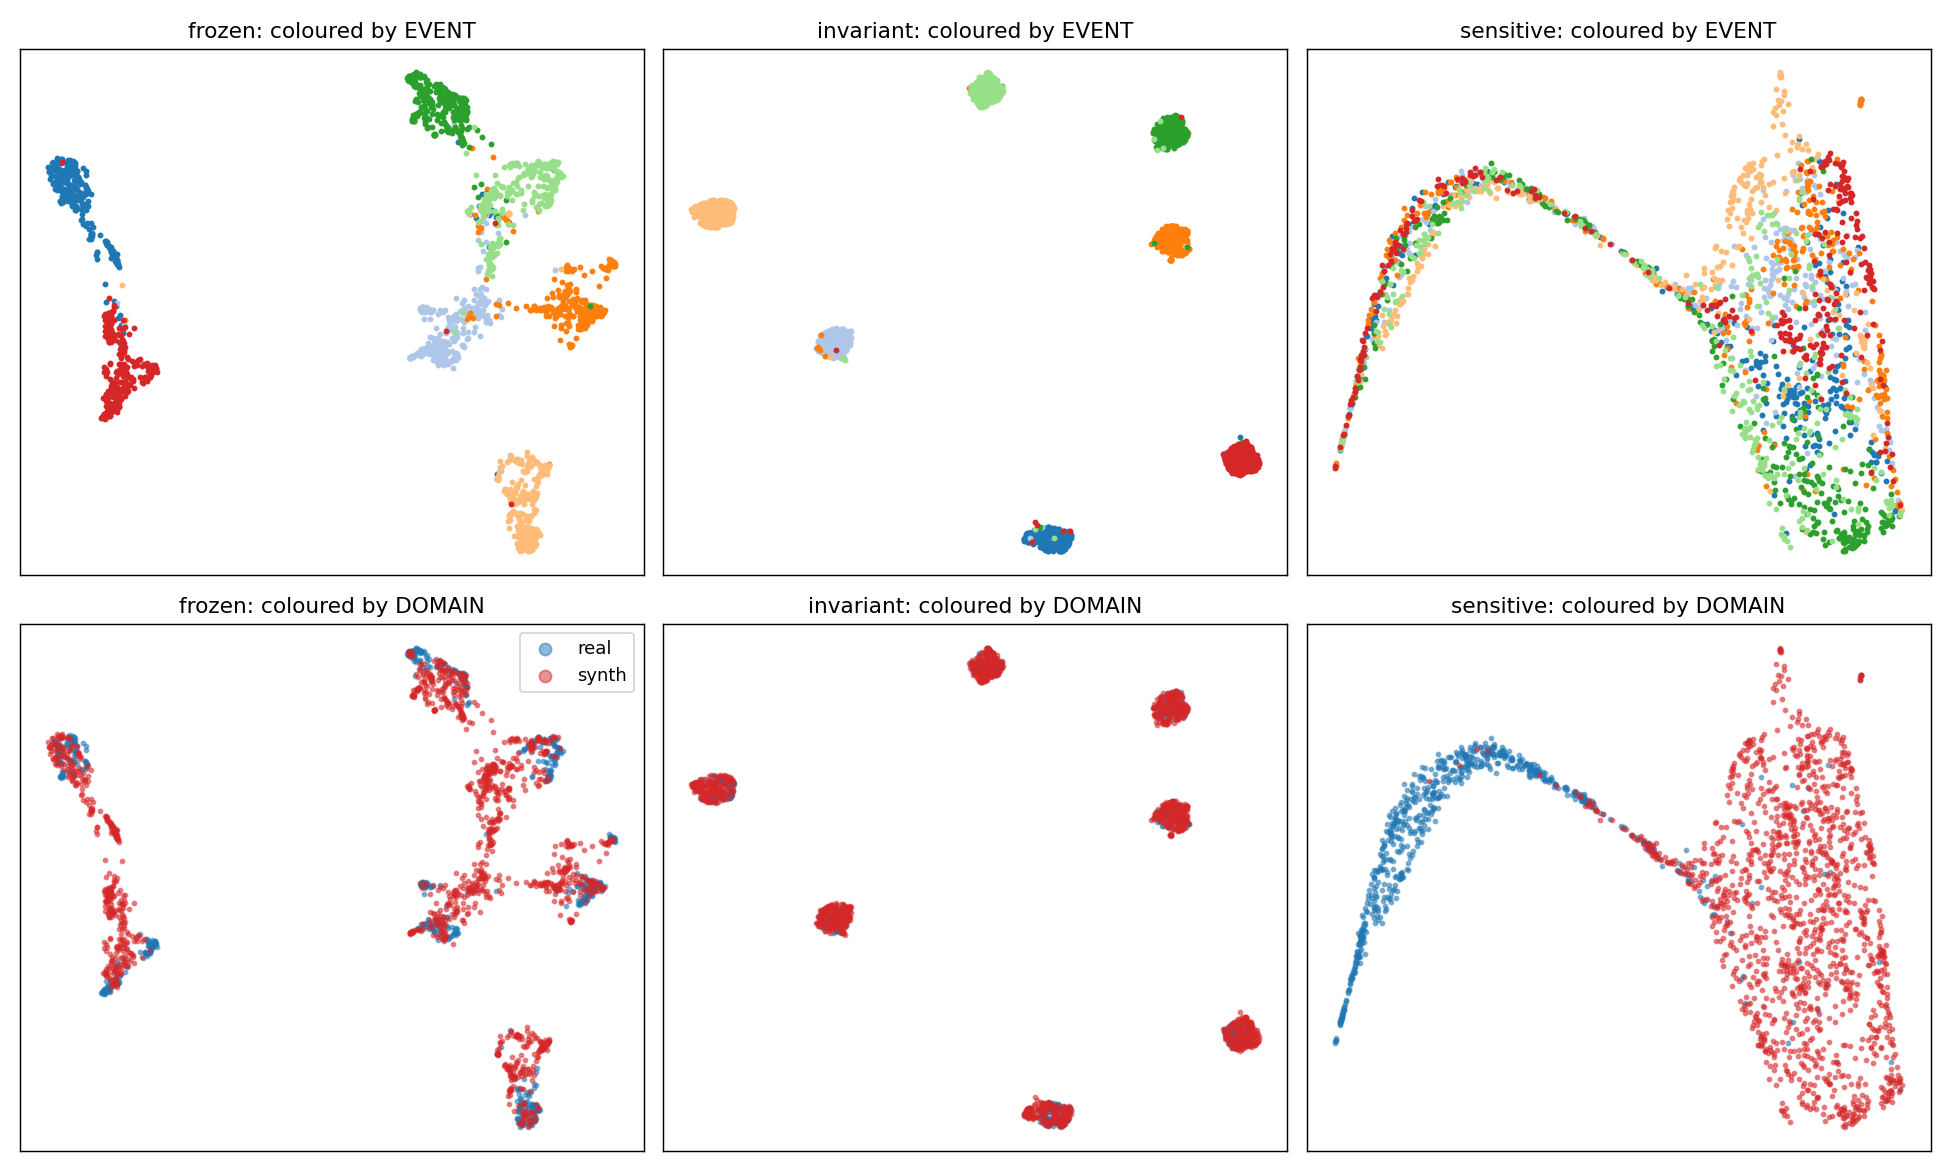
\includegraphics[width=0.92\textwidth]{fig_umap.png}
\caption{UMAP of the DCASE-T7 test set, frozen vs.\ the two heads, coloured by event (top) and by
domain (bottom). The invariant head tightens event clusters with real/synth overlapping within
each; the sensitive head splits real from synth and smears events---the geometry flips.}
\label{fig:umap}
\end{figure}

\paragraph{The closed-world failure.} Holding one class out of training and evaluating on it, the
held-out class collapses \emph{below} frozen (keyboard $0.69\!\to\!0.43$, gunshot $0.81\!\to\!0.31$,
rain $0.75\!\to\!0.30$). Adding categories does not fix it ($34$-class: $0.40\!\to\!0.19$).

\paragraph{The dissociation (Table~\ref{tab:diss}, Fig.~\ref{fig:main}a).}
\label{sec:diss}
Training on the pairs, the instance objective generalizes instance correspondence to categories
unseen \emph{by the head} (the frozen backbone's pretraining is uncontrolled, so ``unseen'' means
not seen during head training). Against the full real test gallery ($N\!=\!3{,}065$ distractors of
\emph{all} categories, chance R@1 $=0.0003$) the instance head retrieves the exact real twin with
R@1 $0.800$ ($[0.786,0.813]$), beating frozen ($0.611$) in all five folds (min margin $+0.148$) and
class-supervision ($0.269$, which \emph{hurts}) in all five (min $+0.493$); no objective transfers
category clustering (all $\le$ frozen on unseen-category mAP). A compute-matched supervised
cross-entropy classifier head fares identically to class-supcon ($0.282$), so the failure is from
training on \emph{class labels}, not from the contrastive form---only instance-pair supervision
generalizes. It holds on three encoders---CLAP,
PANNs, and AST~\citep{gong2021ast} (full-gallery instance R@1 $0.80/0.69/0.93$ vs.\ frozen
$0.58/0.62/0.82$ vs.\ class $0.25/0.32/0.29$; instance $>$ frozen and class $\ll$ frozen on all
three). Two of these (PANNs, AST) did \emph{not} participate in CLAP-verification of the corpus, so
the dissociation is not an artifact of the CLAP filter. (AST's frozen R@1 is already high---these
audio-init twins are near-duplicates for a strong encoder---which is exactly why the
class-supervision \emph{collapse} to $0.29$ is the more informative half of the dissociation.)

\paragraph{Not near-copies (Fig.~\ref{fig:main}b).} Audio-init twins resemble their source, so I
test whether the head merely exploits near-copies: across twin-fidelity levels (the head still
helps, advantage $+0.43..0.52$ over frozen) it holds up and collapses to chance only when the twin
is independent of its source. (This control is measured in CLAP space and is in-domain; the
across-category claim rests on the leave-classes-out result above.)

\paragraph{Cross-generator scope (the claim's boundary).} Adding 670 ElevenLabs (text-only) twins
captioned from each clip's metadata, instance correspondence is weak (frozen R@1 $0.11$ vs.\
$0.55$--$0.98$ for audio-init): the caption is a bottleneck, so the twins are category-appropriate
but not renderings of the \emph{specific} clip. The learned mapping is therefore specific to
\emph{audio-conditioned} generation---it is an instance-correspondence inverse for a given
generator family, not a universal synthetic$\to$real transform.

\begin{table}[t]
\caption{Frozen encoders: synthetic--real gap on DCASE-T7 (test split).}
\label{tab:frozen}
\centering
\begin{tabular}{lccccc}
\toprule
frozen & control & synth$\to$real mAP & gap & PAD & domain-probe \\
\midrule
CLAP        & 0.935 & 0.774\,[0.766,0.783] & $+0.161$ & 1.27 & 0.90 \\
PANNs CNN14 & 0.798 & 0.674                & $+0.124$ & 1.39 & 0.90 \\
\bottomrule
\end{tabular}
\end{table}

\begin{table}[t]
\caption{Five-fold leave-classes-out on the UCS corpus, CLAP, held-out (unseen) categories.
Instance-R@1 is against the \emph{full} real test gallery ($N=3{,}065$, chance $0.0003$); 95\%
bootstrap CIs over queries. category-mAP is full-gallery synth$\to$real category retrieval.}
\label{tab:diss}
\centering
\begin{tabular}{lcc}
\toprule
variant (unseen categories) & category-mAP & \textbf{instance-R@1 (full gallery)} \\
\midrule
frozen        & $0.611$ & $0.611\;[0.594,0.629]$ \\
class-supcon  & $0.459$ & $0.269\;[0.254,0.285]$ \\
class-CE (classifier) & $0.451$ & $0.282\;[0.266,0.297]$ \\
\textbf{instance} & $0.492$ & $\mathbf{0.800\;[0.786,0.813]}$ \\
\bottomrule
\end{tabular}
\end{table}

\begin{figure}[t]
\centering
\begin{subfigure}{0.5\textwidth}\centering
  
\includegraphics[width=\linewidth]{fig_dissociation.png}\caption{}\end{subfigure}%
\begin{subfigure}{0.5\textwidth}\centering
  
\includegraphics[width=\linewidth]{fig_fidelity.png}\caption{}\end{subfigure}
\caption{(a) The instance/category dissociation on unseen categories, three encoders: instance
matching generalizes (left), category retrieval does not (right). (b) Fidelity spectrum: the
instance head holds up as twins diverge from their source.}
\label{fig:main}
\end{figure}

\section{Conclusions, Limitations, and Future Work}
Audio-conditioned synthetic$\to$real instance correspondence is learnable and transfers across
categories; category identity is not, and the correspondence is generator-specific. \textbf{The
central caveat} (stated up front): because the synthetic twins are generated \emph{from} the source
audio, ``retrieve the exact twin'' is closer to cross-domain near-duplicate matching than to
inverting a general rendering process---the ElevenLabs result (text-only twins, R@1 $0.11$) shows
the learned mapping does not transfer to a generator that does not condition on the source.
\textbf{Other limitations}: category clustering does not transfer to unseen categories
(train per target taxonomy); twins are Stable-Audio audio-init at one operating point per corpus;
frozen-embedding heads cannot recover information the backbone discarded; instance pairing requires
audio-conditioned generation; and the UCS corpus is CLAP-verified, which could bias CLAP results
upward---I mitigate this by showing the dissociation holds on PANNs and AST (which did not verify
the corpus), and by noting that the DCASE-T7 gap (Table~\ref{tab:frozen}, an \emph{unverified}
corpus) is comparable. SSL encoders
(BEATs~\citep{chen2023beats}, AudioMAE~\citep{huang2022audiomae}) are provided as activatable loaders. \textbf{Future work}: broader real sources (e.g.\
VGGSound~\citep{chen2020vggsound}) and domain-relevant corpora (game and film SFX), and using the
sensitive head as a realness metric for generative-audio evaluation.

\section*{Reproducibility and release}
Code (MIT), DCASE and UCS manifests, the CLAP-verification, the generation recipe (event, prompt,
seed, steps---bit-reproducible without redistributing restricted audio), the trained heads, and a
reusable transform are released. A datasheet~\citep{gebru2021datasheets} and a persistent
hosting/maintenance plan are in the appendix.

\bibliographystyle{plainnat}
\bibliography{references}

\appendix
\section{Datasheet, hosting, and maintenance}
The appendix provides the Gebru et al.~\citep{gebru2021datasheets} datasheet (motivation,
composition, collection, preprocessing, uses, distribution), per-class/per-split statistics, the
licensing matrix (CC-licensed audio redistributed; BBC and restricted audio shipped as a fetch
manifest plus the generation recipe), and the maintenance plan (versioned manifests; the code
regenerates all derived artifacts from the manifest and the source archives).

\section{Corpus statistics and per-event analysis}
\begin{table}[h]
\caption{Per-domain, per-split clip counts. DCASE-T7 real test is DCASE's source-disjoint eval
set; the UCS corpus uses FSD50K's train/val/eval, uploader-keyed.}
\label{tab:stats}
\centering\small
\begin{tabular}{llccc}
\toprule
corpus & domain & train & val & test \\
\midrule
DCASE-T7 & real  & 4{,}150 & 700 & 700 \\
DCASE-T7 & synth & 18{,}165 & 3{,}884 & 3{,}851 \\
UCS (34 cls) & real  & 8{,}315 & 999 & 4{,}265 \\
UCS (34 cls) & synth (twins) & 6{,}636 & 719 & 3{,}065 \\
\bottomrule
\end{tabular}
\end{table}

\begin{table}[h]
\caption{Per-event frozen-CLAP cross-domain (synth$\to$real) mAP on DCASE-T7. Fast, granular
transient/mechanical sounds transfer worst.}
\label{tab:perevent}
\centering\small
\begin{tabular}{lccccccc}
\toprule
& motor & gunshot & dog\_bark & sneeze & rain & footstep & keyboard \\
\midrule
mAP & 0.852 & 0.810 & 0.809 & 0.793 & 0.752 & 0.718 & 0.692 \\
\bottomrule
\end{tabular}
\end{table}

\begin{figure}[h]
\centering
\begin{subfigure}{0.49\textwidth}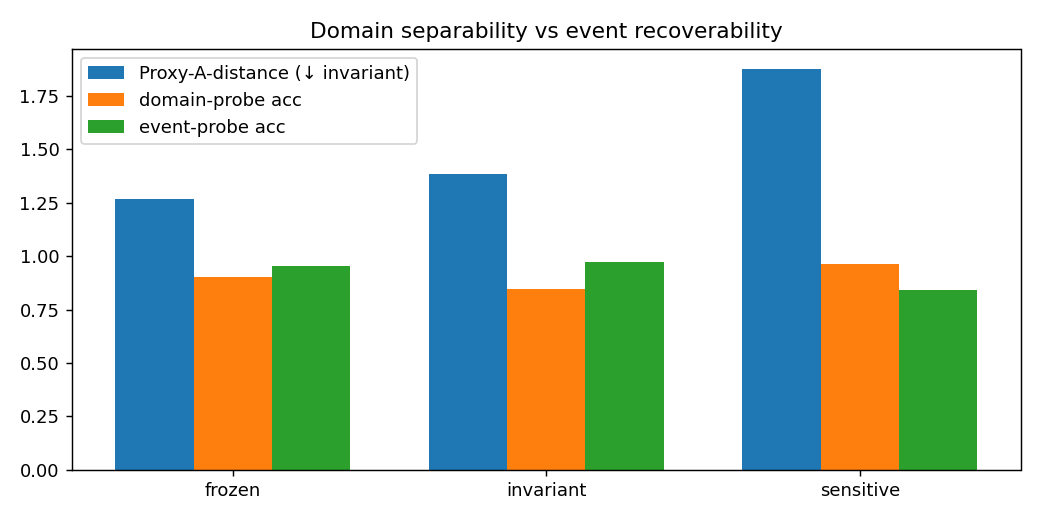
\includegraphics[width=\linewidth]{fig_probes.png}\caption{}\end{subfigure}\hfill
\begin{subfigure}{0.49\textwidth}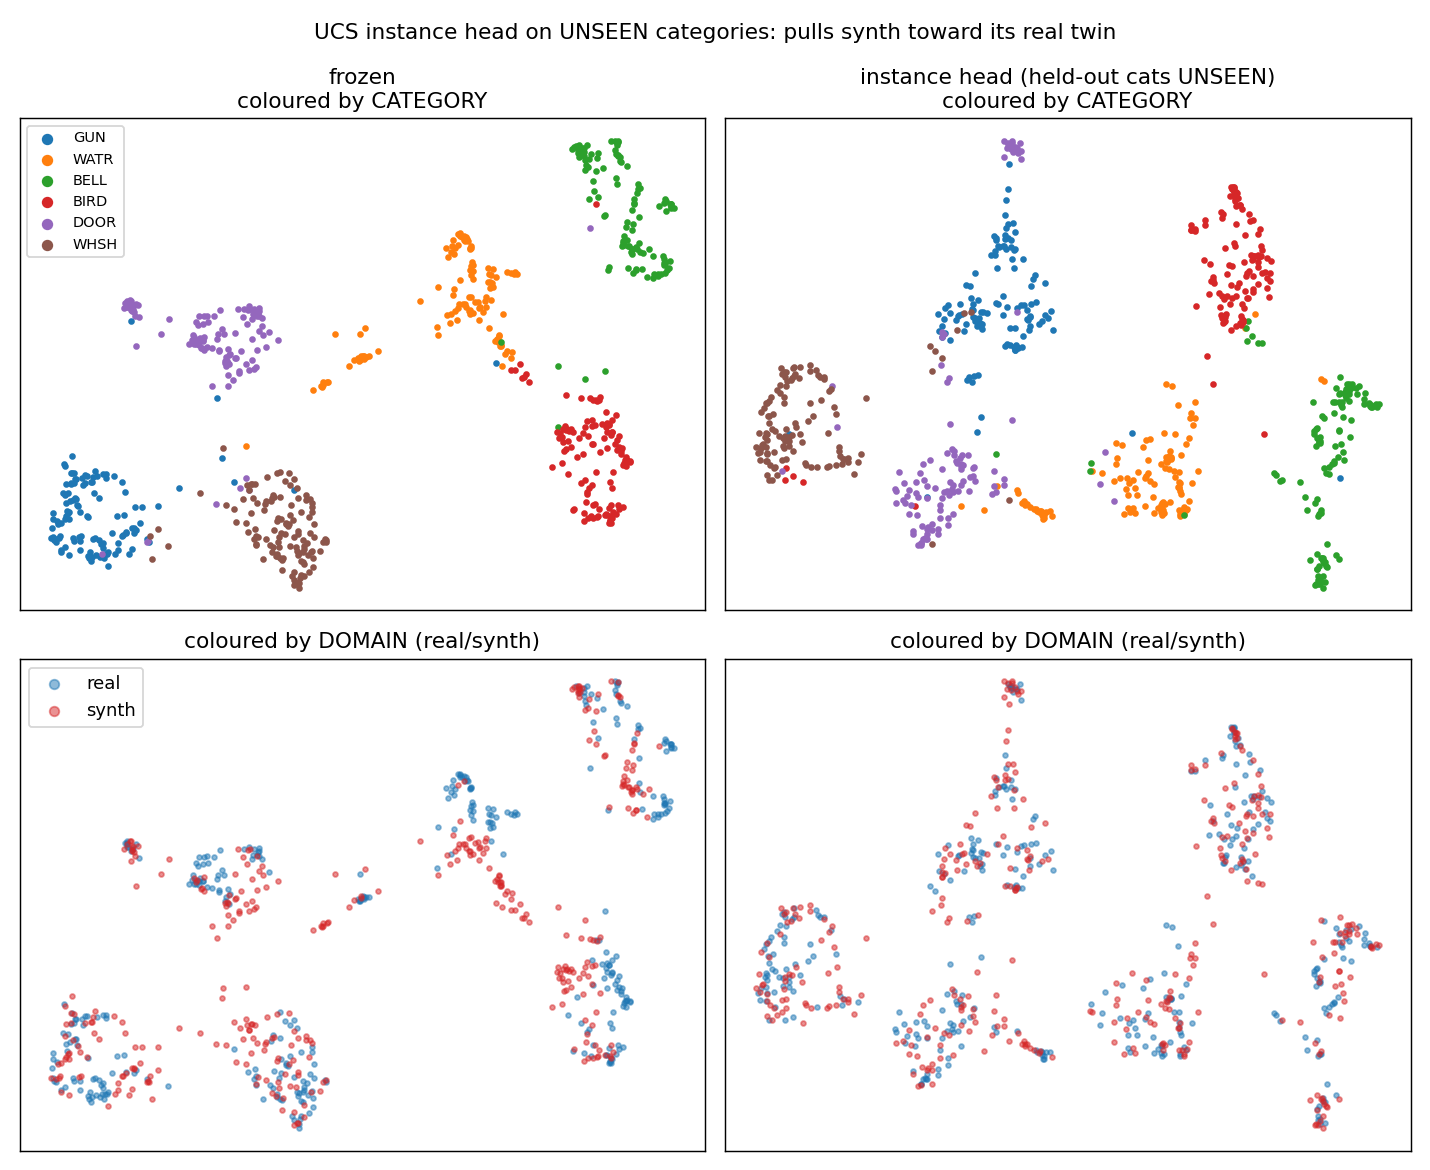
\includegraphics[width=\linewidth]{fig_umap_instance.png}\caption{}\end{subfigure}
\caption{(a) Proxy-A-distance and event/domain linear-probe accuracy across the DCASE heads.
(b) UMAP of the instance head on unseen UCS categories: it mixes real/synth (domain) more than
frozen.}
\label{fig:appendix}
\end{figure}

\end{document}
